\documentclass[a4paper,10pt]{article}
\usepackage[a4paper,hmargin=1.7cm,top=1.8cm,bottom=2.3cm,footskip=1.1cm]{geometry}
\usepackage{times}
\renewcommand{\familydefault}{\sfdefault}
\usepackage[T1]{fontenc}
\usepackage[utf8]{inputenc}
\usepackage[spanish,es-tabla,es-noshorthands]{babel}
\usepackage{amsmath}
\usepackage{multicol}
\usepackage{graphicx}
\usepackage{xcolor}
\usepackage{colortbl}
\usepackage{booktabs}
\usepackage{tabularx}
\usepackage{array}
\usepackage{shadow}
\usepackage{float}
\usepackage{caption}
\usepackage{enumitem}
\usepackage{titlesec}
\usepackage{siunitx}
\sisetup{output-decimal-marker={,}, group-separator={.}, group-minimum-digits=4, mode=text}
\usepackage{textcomp}

\graphicspath{{figuras/}}

\setlength{\parindent}{0pt}
\setlength{\parskip}{0.55em}
\setlength{\columnsep}{0.7cm}
\setlength{\columnseprule}{0.4pt}
\pagestyle{plain}
\setlist[itemize]{leftmargin=1.3em,itemsep=1pt,topsep=2pt}

\definecolor{BoxCol}{rgb}{0.9,0.9,0.9}
\definecolor{propio}{HTML}{2A78D6}
\definecolor{propiofondo}{HTML}{E3EEFB}
\setlength{\sboxrule}{0.6pt}
\setlength{\sboxsep}{0pt}
\setlength{\sdim}{1.6pt}
\newlength{\secboxwidth}
\newcommand{\cajaseccion}[1]{%
  \setlength{\secboxwidth}{\dimexpr\linewidth-0.6cm\relax}%
  \centering
  \shabox{\colorbox{BoxCol}{%
    \begin{minipage}[c]{\secboxwidth}\centering
      \rule{0pt}{2.7ex}\bfseries\large\thesection.~#1\rule[-1.0ex]{0pt}{0pt}%
    \end{minipage}}}}
\titleformat{\section}[block]{}{}{0pt}{\cajaseccion}
\titlespacing*{\section}{0pt}{1.0em plus 0.4em minus 0.2em}{0.3em}

\captionsetup{font=small,labelfont=bf,labelsep=period,skip=6pt}
\captionsetup[table]{position=top}
\renewcommand{\thetable}{\Roman{table}}

\newcolumntype{L}{>{\raggedright\arraybackslash}X}
\newcolumntype{C}[1]{>{\centering\arraybackslash}p{#1}}
\newcolumntype{P}[1]{>{\raggedright\arraybackslash}p{#1}}
\renewcommand{\arraystretch}{1.2}
\newcommand{\ok}{\cellcolor{propiofondo}}          % celda que cumple la meta
\newcommand{\m}{\textminus}                    % signo menos en la letra del texto

\begin{document}

\begin{center}
  {\LARGE\bfseries Resultados de las mediciones del generador\par}
  \vspace{0.7em}
  {\large\bfseries Chantiri, Ignacio Nahuel 69869/1 \quad Fernández Madau, Esteban 71271/5\par}
  \vspace{0.5em}
  {\normalsize Hoja de resultados -- Proyecto Integrador de Electrónica\\[0.2ex]
  Facultad de Ingeniería de la Universidad Nacional de La Plata, 2026\par}
\end{center}
\vspace{0.3em}

\begin{multicols}{2}

\section{Cómo se midió}
La salida de cada canal del DAC del PCM3060 se llevó, a través del capacitor de acople, a la entrada del
mismo canal del ADC del codec (lazo directo). La placa es el prototipo en placa perforada, con la
alimentación analógica del codec separada de la del microcontrolador y las masas unidas en un solo punto.
El ADC muestrea a \SI{97656,25}{Hz} con 24 bits y el microcontrolador envía las muestras a la PC por USB.
Cada captura dura \SI{10}{s}; en las 51 capturas de la sesión no se perdió ninguna trama.

El análisis se hace sobre la transformada de toda la captura con ventana Blackman-Harris. Ruido y
armónicos se integran en la banda de \SI{400}{Hz} a \SI{20}{kHz}, la de la hoja de datos del codec,
y también en \SI{20}{Hz} a \SI{20}{kHz} con y sin ponderación A. La referencia \SI{0}{dBFS} es una
senoidal de fondo de escala. Las medidas de pureza se repitieron tres veces: el THD+N y el SNR no
variaron más de \SI{0,2}{dB}, y en las tablas se informa el promedio.

El ADC es la regla con la que se mide: los resultados son de la cadena completa, DAC más ADC, y
el generador solo nunca puede ser peor que ellos.

\section{Pureza del generador}
Con una senoidal de \SI{1}{kHz} por tabla, al 63\,\% de amplitud (\m{}1,7\,dBFS en el ADC), los dos
canales superan con amplio margen todos los mínimos de la propuesta (Tabla~\ref{tab:pureza}).

\begin{table}[H]
  \caption{Pureza medida con 1\,kHz, en 400\,Hz--20\,kHz, contra las metas de la propuesta. Mínimo:
  criterio de éxito. Techo: típico del DAC del PCM3060. En celeste, lo que cumple el mínimo.}
  \label{tab:pureza}
  \footnotesize
  \begin{tabularx}{\linewidth}{@{}L C{0.12\linewidth}C{0.12\linewidth}C{0.12\linewidth}C{0.12\linewidth}@{}}
  \toprule
  \textbf{Parámetro} & \textbf{Mínimo} & \textbf{Techo} & \textbf{L} & \textbf{R} \\
  \midrule
  THD+N [dB]            & \textless\,\m{}60 & \m{}94 & \ok\m{}90,1 & \ok\m{}89,8 \\
  THD [dB]              & --     & --    & \m{}100,3   & \m{}106,4 \\
  SNR [dB]              & \textgreater\,80  & 105   & \ok90,5  & \ok89,9 \\
  SFDR [dB]             & \textgreater\,70  & --    & \ok100,4 & \ok99,8 \\
  ENOB [bits]           & --     & --    & 14,7         & 14,6 \\
  Separación [dB]       & \textgreater\,80  & 103   & \ok124,8 & \ok\textgreater\,128 \\
  \bottomrule
  \end{tabularx}
\end{table}

El THD+N de \m{}90\,dB (0,003\,\%) está limitado por el ruido y no por la distorsión: el segundo
armónico queda \SI{104}{dB} por debajo del fondo de escala (Figura~\ref{fig:espectro}). Es lo esperable
de la cadena: combinando los valores típicos del DAC (\m{}94\,dB) y del ADC (\m{}93\,dB) resultan
\m{}90,5\,dB, así que la cadena rinde lo que promete el fabricante. Por eso el techo de la tabla, que
es del DAC solo, no se puede verificar con esta regla. La separación de R hacia L queda al nivel del
ruido: el cruce no llega a verse.

\begin{figure}[H]
  \centering
  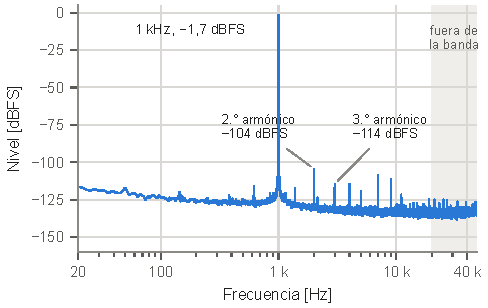
\includegraphics[width=\linewidth]{espectro_tabla_1k.pdf}
  \caption{Espectro del canal L con 1\,kHz por tabla al 63\,\%. El piso por bin depende de la
  resolución (1,5\,Hz); el ruido integrado en la banda es de \m{}95,5\,dBFS.}
  \label{fig:espectro}
\end{figure}

\section{Tabla contra acumulador de fase}
La pregunta central de la propuesta era si la síntesis por acumulador, que permite cualquier frecuencia,
alcanza la pureza necesaria, o si conviene una tabla de frecuencia fija. Se midió la misma senoidal de
1\,kHz por los dos métodos, alternándolos tres veces sin tocar el montaje (Tabla~\ref{tab:sintesis}).

\begin{table}[H]
  \caption{Senoidal de 1\,kHz por acumulador de fase y por tabla, canal L, 400\,Hz--20\,kHz.}
  \label{tab:sintesis}
  \footnotesize
  \begin{tabularx}{\linewidth}{@{}L C{0.2\linewidth}C{0.2\linewidth}@{}}
  \toprule
  \textbf{Parámetro} & \textbf{Acumulador} & \textbf{Tabla} \\
  \midrule
  THD+N [dB]                     & \m{}74,8 & \m{}90,0 \\
  SNR [dB]                       & 74,8      & 90,5 \\
  SFDR [dB]                      & 78,3      & 100,4 \\
  Mayor espuria no armónica [dBc] & \m{}78,3 & \m{}114,9 \\
  \bottomrule
  \end{tabularx}
\end{table}

El acumulador produce las espurias de truncación de fase que preveía la teoría: las dos mayores, en
10,1 y 12,1\,kHz, quedan a \m{}78\,dBc, el valor calculado en la propuesta (Figura~\ref{fig:sintesis}).
Su energía se suma al ruido y le cuesta \SI{15}{dB} de THD+N respecto de la tabla. Aun así, el
acumulador cumple con holgura los mínimos de THD+N y SFDR; la tabla, en cambio, lleva la pureza
hasta el límite del codec.

\begin{figure}[H]
  \centering
  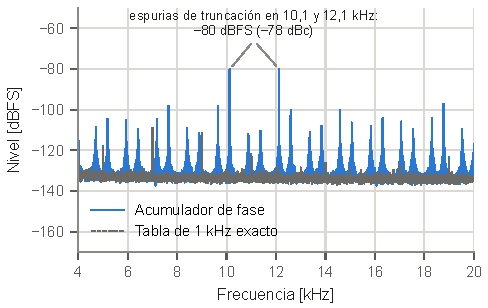
\includegraphics[width=\linewidth]{acumulador_vs_tabla.pdf}
  \caption{Espectro entre 4 y 20\,kHz de la misma senoidal de 1\,kHz por los dos métodos.}
  \label{fig:sintesis}
\end{figure}

En el peor caso de truncación (995,4\,Hz con el paso de fase más desfavorable) la espuria aparece en
\SI{47,8}{kHz} a \m{}81\,dBc, fuera de la banda de audio; con la tabla, a la misma frecuencia, no se
distingue del ruido (\m{}126\,dBc).

\section{Ruido, rango dinámico y linealidad}

\begin{table}[H]
  \caption{Ruido, rango dinámico y amplitud. DR: rango dinámico, ponderado A.}
  \label{tab:ruido}
  \footnotesize
  \begin{tabularx}{\linewidth}{@{}L C{0.17\linewidth}C{0.17\linewidth}@{}}
  \toprule
  \textbf{Parámetro} & \textbf{L} & \textbf{R} \\
  \midrule
  Piso de ruido, 400\,Hz--20\,kHz [dBFS]  & \m{}95,5 & \m{}95,1 \\
  Piso de ruido, 20\,Hz--20\,kHz [dBFS]   & \m{}94,9 & \m{}94,3 \\
  DR, método EIAJ (señal a \m{}60\,dB) [dB] & 96,8      & 96,4 \\
  Nivel al 63\,\% de amplitud [dBFS]       & \m{}1,72 & \m{}1,53 \\
  Error de los escalones de 6\,dB [dB]     & \multicolumn{2}{c}{$\le$\,0,04} \\
  Intermodulación 60\,Hz + 7\,kHz [dBc]    & \multicolumn{2}{c}{\m{}98} \\
  \bottomrule
  \end{tabularx}
\end{table}

Con el DAC encendido en silencio, el piso de la cadena queda en \m{}95\,dBFS y no aparece zumbido de
red. El rango dinámico de 96,6\,dB (A) supera el mínimo garantizado del ADC (95\,dB) y queda a 2,5\,dB
de su valor típico (99\,dB). La amplitud se controla en pasos exactos: al bajar de 63\,\% a 8\,\%, cada
escalón de 6\,dB se cumple con un error menor que 0,04\,dB. Con dos tonos simultáneos la cadena no los
mezcla: los productos de intermodulación quedan 98\,dB por debajo.

\section{Lo que se aprendió al medir}
\begin{itemize}
  \item \textbf{La alimentación compartida metía el ruido digital.} Con el codec alimentado desde el USB
  del microcontrolador, el piso era de \m{}57\,dBFS, dominado por una línea en 381,5\,Hz: la frecuencia
  a la que el programa arma y envía cada paquete de 256 muestras. Al cambiar el paquete a 512 muestras
  la línea se mudó a 190,7\,Hz, y al separar la alimentación desapareció. Es la razón de la entrada
  de alimentación analógica separada en el circuito impreso.
  \item \textbf{El dato del ADC llega a veces corrido un bit.} Según el armado, el I2S del
  microcontrolador recibe la muestra desplazada un bit o no. El programa lo detecta solo en cada
  bloque y lo corrige; en esta sesión el dato llegó bien alineado.
  \item \textbf{El USB de algunas PC no alcanza para los dos canales.} En una de las PC se perdía el
  4\,\% de las tramas en estéreo, así que se midió un canal por vez y la separación se obtuvo de
  capturas del otro canal con el tono sonando.
\end{itemize}

\section{Condiciones y pendientes}
La frecuencia de muestreo usada (97,66\,kHz) está algo por encima del máximo del ADC según su hoja de
datos (96\,kHz), y los valores típicos del fabricante están dados a 48\,kHz: la comparación es
aproximada. Quedan por medir con instrumental la exactitud de frecuencia, la amplitud de salida en
volts y las formas de onda.

\end{multicols}
\end{document}
